\section{Operationen}
Nachdem ein Half-Edge Mesh prozedural erstellt wurde oder ein Unity Mesh umgewandelt wurde, k\"onnen auf ein Half-Edge Mesh einige Standardoperationen angewendet werden. Folgende Operationen werden im folgenden Kapitel erkl\"art und die Implementierung beschrieben:
\begin{itemize}
	\item das Teilen einer HalfEdge (Split HalfEdge),
	\item das Kollabieren einer Kante (Edge Collapse),
	\item das Aufteilen einer Face (Subdivision) und
	\item eine einfache 2D-Zerst\"orungssimulation (Simulate Breaking).
\end{itemize}

\subsection{Split Half-Edge}
Ziel der \textit{SplitHalfEdge}-Methode ist es, eine HalfEdge so zu teilen, dass das Ergebnis der Operation ein konformes Half-Edge Mesh ist, also dass jede Face immer noch aus drei Half-Edges besteht und dass jede Half-Edge maximal einen Partner besitzt. Um das Teilen durchzuf\"uhren, m\"ussen folgende Schritte durchgef\"uhrt werde, die in der Abbildung \ref{fig:splithalfedge} schematisch dargestellt sind:
\begin{enumerate}
	\item Bestimme die zu splittende HalfEdge.
	\item Erzeuge einen neuen Punkt, dort wo sich die HalfEdge aufteilt.
	\item Erzeuge drei neue HalfEdges und eine neue Face:
	\begin{itemize}
		\item Eine HalfEdge zum neuen Punkt, vom Ursprung der gesplitteten HalfEdge
		\item Eine HalfEdge als Nachfolger der ersten HalfEdge, mit dem neuen Punkt als Ursprung 
		\item Eine HalfEdge als Vorg\"anger der gesplitteten HalfEdge
	\end{itemize}
	\item Setze die Referenzen der HalfEdges neus
	\item F\"uhre Schritte 1-4 f\"ur die der gesplitteten HalfEdge gegen\"uberliegende HalfEdge ebenfalls aus
	\item Setze die Paare neu
\end{enumerate}

\begin{figure}[H]
	\centering
	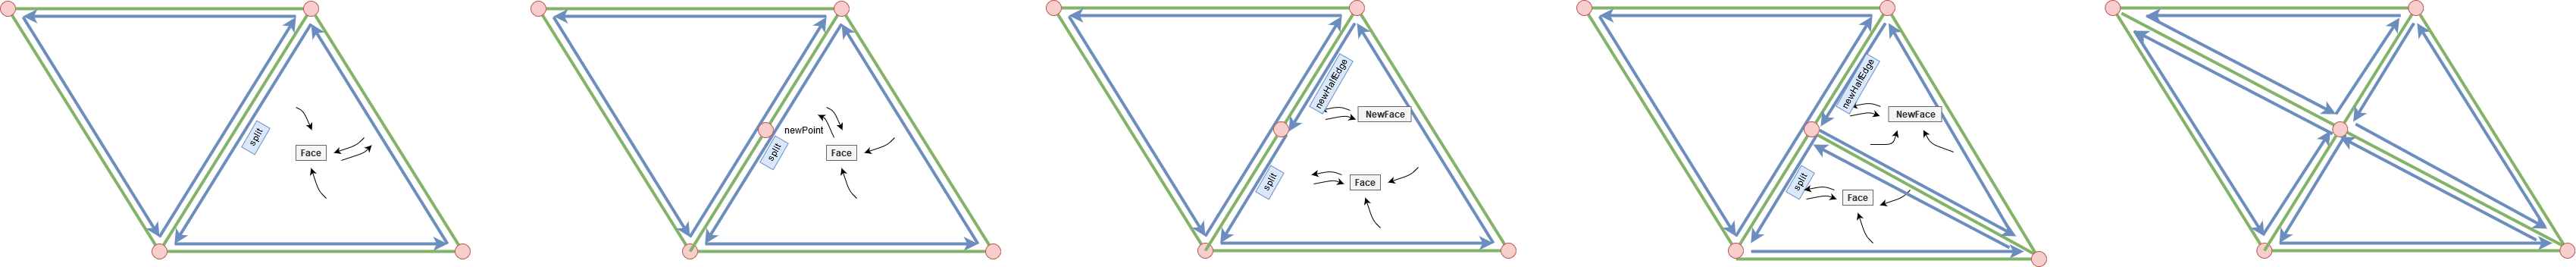
\includegraphics[width=1\linewidth]{Images/splitHalfEdge}
	\caption{Schematische Darstellung eines Edge splits. In Bild 1 ist die Ausgangssituation, Bild 2 zeigt Schritt 2, die Bilder 3 und 4 zeigen die Schritte 3 und 4 und Bild 5 zeigt das Ergebnis, nach den Schritten 5 und 6.}
	\label{fig:splithalfedge}
\end{figure}


Der beschriebene Algorithmus besitzt eine konstante Laufzeit, da die einzigen ,,komplexen'' Operationen auf der \textit{GetFaceCirculator}-Methode basieren, die immer die drei anliegenden HalfEdges einer Face zur\"uckgibt. Er ist im Folgenden implementiert:
\begin{lstlisting}
private bool _lock = false;
private HalfEdge _newHalfEdge, _split;

public void SplitHalfEdge(HalfEdge split, Vector3 splitPoint)
{
	// --- Schritt 1:
	split.Face.HalfEdge = split; // --- Set Reference of 
	// --- Face to split to know where the new face goes
	_split = split;

	// --- Schritt 2:
	Vertex newPoint = _mesh.Vertices.CreateVertex(splitPoint);

	// --- Schritt 3:
	HalfEdge newHalfEdge = _mesh.HalfEdges
	.CreateHalfEdge(split.OutgoingPoint, null, split);
	_newHalfEdge = newHalfEdge;
	Face newFace = _mesh.Faces.CreateFace(newHalfEdge);
	split.OutgoingPoint = newPoint;

	HalfEdge newHalfEdgeToSplit = _mesh.HalfEdges
	.CreateHalfEdge(split.Next.EndPoint, split.Face, split);
	HalfEdge newHalfEdgeFromNewHalfEdge = _mesh.HalfEdges
	.CreateHalfEdge(newPoint, newFace, split.Next.Next);
	_mesh.HalfEdges
	.CreatePair(newHalfEdgeToSplit, newHalfEdgeFromNewHalfEdge);

	// --- Schritt 4:
	newHalfEdge.Next = newHalfEdgeFromNewHalfEdge;
	newHalfEdgeFromNewHalfEdge.Next.Next = newHalfEdge;
	split.Next.Next = newHalfEdgeToSplit;

	// --- Aktualisiere das Unity Mesh
	_mesh.AddMeshVertex(newPoint.Point);
	
	_mesh.SetMeshTriangles(split.Face.Index,
	_mesh.Faces.GetFaceCirculator(split.Face)
	.Select(p => p.OutgoingPoint.Index)
	.ToList(), true);
	 
	_mesh.SetMeshTriangles(newFace.Index,
	_mesh.Faces.GetFaceCirculator(newFace)
	.Select(p => p.OutgoingPoint.Index)
	.ToList(), true);
	
	if (!_lock) // --- Blockiere nach dem ersten Aufruf,
				// --- um eine Endlosschleife zu vermeiden
	{
		// --- Schritt 5:
		if (split.Opposing != null) 
		{
			_lock = true;
			SplitHalfEdge(split.Opposing, splitPoint);
			// --- Schritt 6:
			_mesh.HalfEdges.CreatePair(_split, newHalfEdge);
			_mesh.HalfEdges.CreatePair(split, _newHalfEdge);
			_lock = false;
		}
	_mesh.CommitMeshTriangles();
	}
}
\end{lstlisting}
In wird die \textit{SplitHalfEdge}-Methode auf das erste Mesh in Abbildung \ref{fig:meshmash} angewendet, so ist das Mesh im zweite Bild das Ergebnis, wenn die Diagonale gesplittet wird und im Dritten, wenn die linke Kante unterhalb der Mitte geteilt wird. Das letzte Bild zeigt, dass der Teilungspunkt nicht zwingend auf der Kante liegen muss, da sich die Kanten entsprechend anpassen.
\begin{figure}[H]
	\centering
	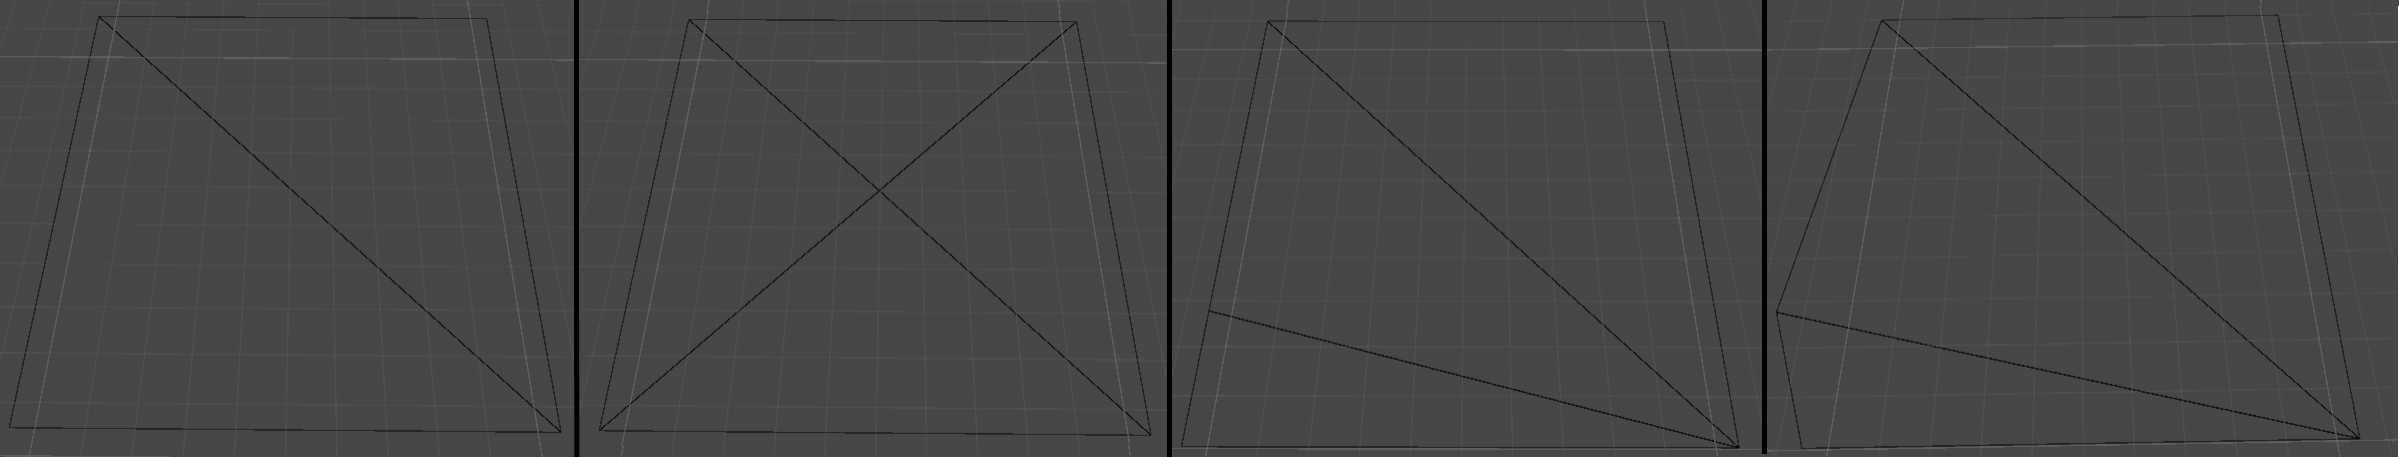
\includegraphics[width=1 \linewidth]{Images/meshmash}
	\caption{Bild 1 ist das Ausgangsmesh, welches in Bild 2 in der Mitte der Diagonale gesplittet wurde, in Bild 3 ein viertel auf dem Weg nach oben, auf der linken Seite und im 4. Bild eine Einheit links von der Kante}
	\label{fig:meshmash}
\end{figure}
